\documentclass[10pt,twocolumn,letterpaper]{article}
\usepackage{cvpr}
\usepackage{times}
\usepackage{epsfig}
\usepackage{graphicx}
\usepackage{amsmath}
\usepackage{amssymb}
\usepackage[breaklinks=true,bookmarks=false,backref=page]{hyperref}
\cvprfinalcopy
\def\cvprPaperID{****}
\def\httilde{\mbox{\tt\raisebox{-.5ex}{\symbol{126}}}}
\begin{document}
\title{\textbf{Image Question Answering using Convolutional Neural Network with Dynamic Parameter Prediction
}}
\author{Liangjie Cao\\\\ Jun 22, 2018}
\maketitle
\abstract{The authors tackle image question answering (ImageQA) problem by learning a convolutional neural network (CNN) with a dynamic parameter layer whose weights are determined adaptively based on questions. For the adaptive parameter prediction, they employ a separate parameter prediction network, which consists of gated recurrent unit (GRU) taking a question as its input and a fully-connected layer generating a set of candidate weights as its output. However, it is challenging to construct a parameter prediction network for a large number of parameters in the fully-connected dynamic parameter layer of the CNN. We reduce the complexity of this problem by incorporating a hashing technique, where the candidate weights given by the parameter prediction network are selected using a predefined hash function to determine individual weights in the dynamic parameter layer. The proposed network��joint network with the CNN for ImageQA and the parameter prediction network�� is trained end-to-end through back-propagation, where its weights are initialized using a pre-trained CNN and GRU. The proposed algorithm illustrates the state-of-the-art performance on all available public ImageQA benchmarks.}
\section{Introduction}
One of the ultimate goals in computer vision is holistic scene understanding~\cite{name30}, which requires a system to capture various kinds of information such as objects, actions, events, scene, atmosphere, and their relations in many different levels of semantics. Although significant progress on various recognition tasks~\cite{name5,name8,name21,name24,name26,name27,name31} has been made in recent years, these works focus only on solving relatively simple recognition problems in controlled settings, where each dataset consists of concepts with similar level of understanding (e.g. object, scene, bird species, face identity, action, texture etc.). There have been less efforts made on solving various recognition problems simultaneously, which is more complex and realistic, even though this is a crucial step toward holistic scene understanding.
\begin{figure}[!htb]
 \centering
 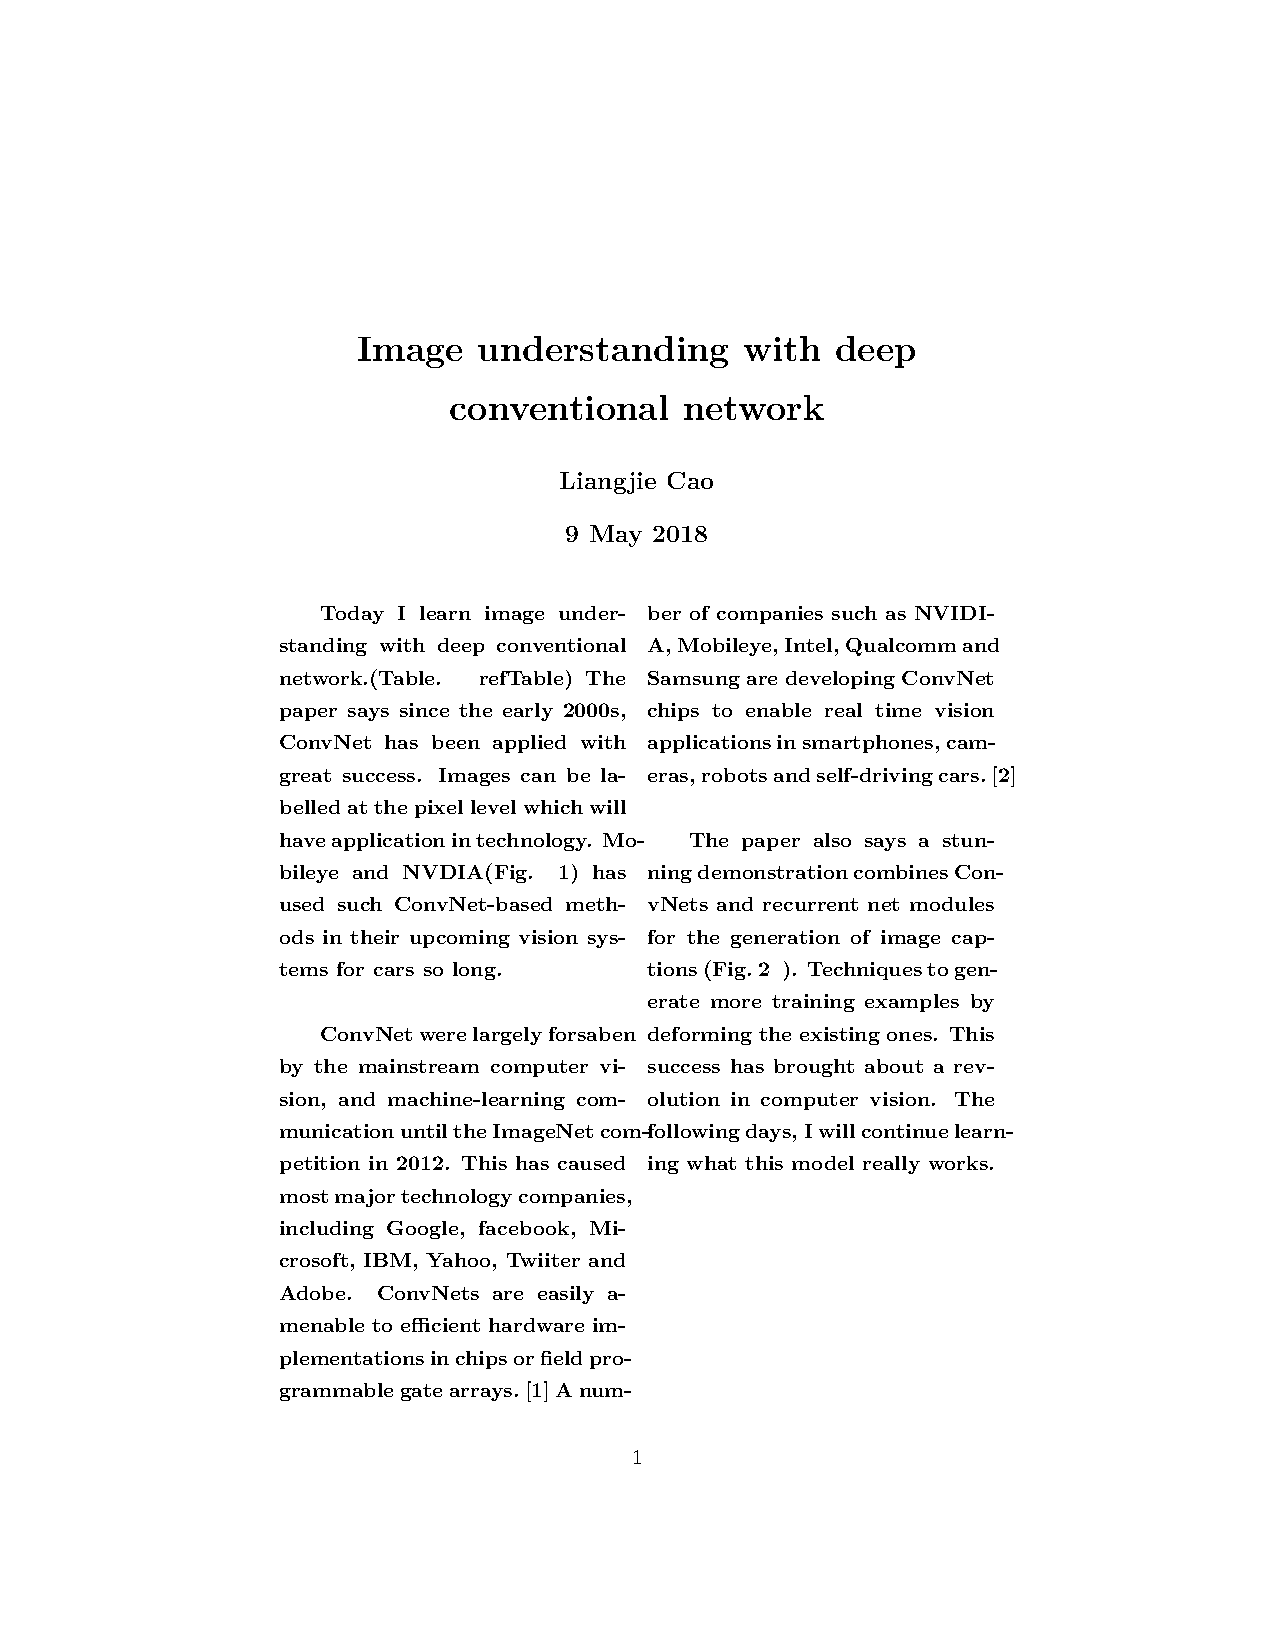
\includegraphics[width=0.5\textwidth]{image.png}\\
 \caption{Sample images and questions in VQA dataset!\cite{name1}. Each question requires different type and/or level of understanding of the corresponding input image to find correct answers}\label{Figure1}
 \end{figure}
\par Image question answering (ImageQA)~\cite{name1} aims to solve the holistic scene understanding problem by proposing a task unifying various recognition problems. ImageQA is a task automatically answering the questions about an input image as illustrated in Figure~\ref{Figure1}. The critical challenge of this problem is that different questions require different types and levels of understanding of an image to find correct answers. For example, to answer the question like ``how is the weather?" they need to perform classification on multiple choices related to weather, while they should decide between yes and no for the question like ``is this picture taken during the day?" For this reason, not only the performance on a single recognition task but also the capability to select a proper task is important to solve ImageQA problem.
\par Contrary to the existing approaches, the authors define a different recognition task depending on a question. To realize this idea, they propose a deep CNN with a dynamic parameter layer whose weights are determined adaptively based on questions. They claim that a single deep CNN architecture can take care of various tasks by allowing adaptive weight assignment in the dynamic parameter layer. For the adaptive parameter prediction, they employ a parameter prediction network, which consists of gated recurrent units (GRU) taking a question as its input and a fully-connected layer generating a set of candidate weights for the dynamic parameter layer. The entire network including the CNN for ImageQA and the parameter prediction network is trained end-to-end through back-propagation, where its weights are initialized using pre-trained CNN and GRU.
\section{Problem Formulation}
ImageQA systems predict the best answer $\hat{a}$ given an image $I$ and a question $q$. Conventional approaches~\cite{name16,name23} typically construct a joint feature vector based on two inputs $I$ and $q$ and solve a classification problem for ImageQA using the following equation:
\begin{equation}
\hat{a}=\mathop{\arg\min}_{a\in\Omega}p(a\mid{I},q;\theta)
\end{equation}
\par where $\Omega$ is a set of all possible answers and $\theta$ is a vector for the parameters in the network. On the contrary, they use the question to predict weights in the classifier and solve the problem. They find the solution by
\begin{equation}
\hat{a}=\mathop{\arg\max}_{a\in\Omega}p(a\mid{I};\theta_{s},\theta_{d}(q))
\end{equation}
\par where $\theta_{s}$ and $\theta_{d}(q)$ denote static and dynamic parameters, respectively. Note that the values of $\theta_{d}(q)$ are determined by the question $q$.
\bibliographystyle{abbrv}
\bibliography{yinyong6}
\end{document}

